  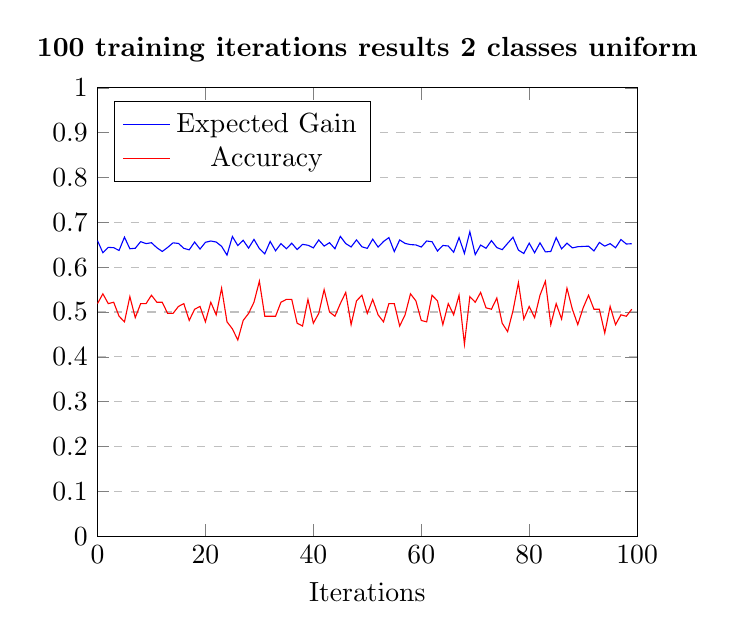
\begin{tikzpicture}
  \begin{axis}[
      title=\textbf{100 training iterations results 2 classes uniform},
      xlabel={Iterations},
      xmin=0, xmax=100,
      ymin=0.0, ymax=1,
      xtick={0,20,40,60,80,100},
      ytick={0.0,0.1,0.2,0.3,0.4,0.5,0.6,0.7,0.8,0.9,1.0},
      legend pos=north west,
      ymajorgrids=true,
      grid style=dashed,
  ]
  
  \addplot[color=blue, mark=dot]
    coordinates {
      (0,0.6593504287948415)
      (1,0.6322952653288357)
      (2,0.6442318074145162)
      (3,0.643532034044156)
      (4,0.6374052549173173)
      (5,0.6670332218794528)
      (6,0.641154535217185)
      (7,0.6422862876918007)
      (8,0.6569850006437995)
      (9,0.6526304654809094)
      (10,0.6546187941166898)
      (11,0.643475265753768)
      (12,0.6351244529764057)
      (13,0.6440720167792894)
      (14,0.6543635532964378)
      (15,0.6530730475972332)
      (16,0.6420652888245892)
      (17,0.6386933525793097)
      (18,0.656131766987587)
      (19,0.6404145019838194)
      (20,0.6554970068445349)
      (21,0.6584519948176737)
      (22,0.6561351500294403)
      (23,0.6465710312484481)
      (24,0.626949097769329)
      (25,0.6684014850794588)
      (26,0.6483354163282329)
      (27,0.6599595111517538)
      (28,0.6425754096484391)
      (29,0.6620319415019925)
      (30,0.6414724731267122)
      (31,0.6298445580096735)
      (32,0.6574631542543048)
      (33,0.636646465705065)
      (34,0.652624576567283)
      (35,0.6411972586281364)
      (36,0.6534335196235858)
      (37,0.6393938870373085)
      (38,0.6509773178827621)
      (39,0.6490233939471659)
      (40,0.643113898351353)
      (41,0.6607874477644926)
      (42,0.6471172254570899)
      (43,0.654665306156185)
      (44,0.6411259548443401)
      (45,0.6688035174036389)
      (46,0.6527749164324254)
      (47,0.6451812873875673)
      (48,0.6609176253324267)
      (49,0.6455335437954625)
      (50,0.642030208545801)
      (51,0.6625253099129024)
      (52,0.6448123479184392)
      (53,0.6573237510186837)
      (54,0.6660459563843424)
      (55,0.6347781754371478)
      (56,0.6607545630657751)
      (57,0.653058954580872)
      (58,0.6504531480193392)
      (59,0.6496864896714141)
      (60,0.6450361030416386)
      (61,0.6584978551443268)
      (62,0.656776335109375)
      (63,0.6360751668081185)
      (64,0.6484932840997125)
      (65,0.6473239417545021)
      (66,0.6334378696365125)
      (67,0.666011299572501)
      (68,0.6307919371924887)
      (69,0.6792398937360165)
      (70,0.6280587830300347)
      (71,0.6494227084162714)
      (72,0.6421450141129107)
      (73,0.6592853024018064)
      (74,0.6438241420702857)
      (75,0.6390998573461351)
      (76,0.6531458725375711)
      (77,0.6668077654917725)
      (78,0.6381550986287792)
      (79,0.630587235329701)
      (80,0.6536501637107353)
      (81,0.6321964946958653)
      (82,0.6543359998085868)
      (83,0.6341080534790973)
      (84,0.6351134667290098)
      (85,0.6659623301074993)
      (86,0.640896953425713)
      (87,0.6535639491294327)
      (88,0.6430701364374961)
      (89,0.6456856464475672)
      (90,0.6463538396337825)
      (91,0.6468890996036903)
      (92,0.636325143508721)
      (93,0.6551562243985622)
      (94,0.6470567257969099)
      (95,0.6525617299247326)
      (96,0.6433204718667557)
      (97,0.6617591734108166)
      (98,0.6517035403538808)
      (99,0.652466037775164)
    };
    \addlegendentry{Expected Gain}
  
  \addplot[color=red]
    coordinates {
      (0,0.51875)
      (1,0.540625)
      (2,0.51875)
      (3,0.521875)
      (4,0.490625)
      (5,0.478125)
      (6,0.534375)
      (7,0.4875)
      (8,0.51875)
      (9,0.51875)
      (10,0.5375)
      (11,0.521875)
      (12,0.521875)
      (13,0.496875)
      (14,0.496875)
      (15,0.5125)
      (16,0.51875)
      (17,0.48125)
      (18,0.50625)
      (19,0.5125)
      (20,0.478125)
      (21,0.521875)
      (22,0.49375)
      (23,0.553125)
      (24,0.478125)
      (25,0.4625)
      (26,0.4375)
      (27,0.48125)
      (28,0.496875)
      (29,0.521875)
      (30,0.56875)
      (31,0.490625)
      (32,0.490625)
      (33,0.490625)
      (34,0.521875)
      (35,0.528125)
      (36,0.528125)
      (37,0.475)
      (38,0.46875)
      (39,0.528125)
      (40,0.475)
      (41,0.496875)
      (42,0.55)
      (43,0.5)
      (44,0.490625)
      (45,0.51875)
      (46,0.54375)
      (47,0.471875)
      (48,0.525)
      (49,0.5375)
      (50,0.496875)
      (51,0.528125)
      (52,0.49375)
      (53,0.478125)
      (54,0.51875)
      (55,0.51875)
      (56,0.46875)
      (57,0.49375)
      (58,0.540625)
      (59,0.525)
      (60,0.48125)
      (61,0.478125)
      (62,0.5375)
      (63,0.525)
      (64,0.471875)
      (65,0.51875)
      (66,0.49375)
      (67,0.5375)
      (68,0.428125)
      (69,0.534375)
      (70,0.521875)
      (71,0.54375)
      (72,0.509375)
      (73,0.50625)
      (74,0.53125)
      (75,0.475)
      (76,0.45625)
      (77,0.503125)
      (78,0.565625)
      (79,0.484375)
      (80,0.5125)
      (81,0.4875)
      (82,0.5375)
      (83,0.56875)
      (84,0.471875)
      (85,0.51875)
      (86,0.484375)
      (87,0.553125)
      (88,0.50625)
      (89,0.471875)
      (90,0.509375)
      (91,0.5375)
      (92,0.50625)
      (93,0.50625)
      (94,0.453125)
      (95,0.5125)
      (96,0.471875)
      (97,0.49375)
      (98,0.490625)
      (99,0.50625)
    };
    \addlegendentry{Accuracy} 
  \end{axis}
\end{tikzpicture}
